%%%%%%%%%%%%%%%%%%%%%%%%%%%%%%%%%%%%%%%%%%%%%%%%%%%%%%%%%%%%%%%%%%%%%%%%%%%%%%%
%% Dokumentation für Praxisprojekt                                           %%
%% (TH Köln -Campus Gummersbach, Fak. 10)                                    %%
%%                                                                           %%
%% 2014-2017                            %%
%%%%%%%%%%%%%%%%%%%%%%%%%%%%%%%%%%%%%%%%%%%%%%%%%%%%%%%%%%%%%%%%%%%%%%%%%%%%%%%

%%%%%%%%%%%%%%%%%%%%%%%%%%%%%%%%%%%%%%%%%%%%%
%% HEADER                                  %%
%%%%%%%%%%%%%%%%%%%%%%%%%%%%%%%%%%%%%%%%%%%%%
\documentclass[a4paper,12pt,oneside]{article}
% Optionen:
% - a4paper => DIN A4-Format
% - 12pt    => Schriftgröße (weitere  
%              grundlegende Fontgrößen: 10pt, 11pt)
% - oneside => Einseitiger Druck

%% Verwendete Pakete:
\usepackage[ngerman]{babel} % für die deutsche Sprache
\usepackage{caption} % Für schönere Bildunterschriften
\usepackage[T1]{fontenc} % Schriftkodierung (Für Sonderzeichen u.a.)
\usepackage[utf8]{inputenc} % Für die direkte Eingabe von Umlauten im Editor u.a.
\usepackage{fancyhdr} % Für Kopf- und Fußzeilen
\usepackage{lscape} % Für Querformat




%% Show code in a better way
\usepackage{listings}
\usepackage{color}

\definecolor{dkgreen}{rgb}{0,0.6,0}
\definecolor{gray}{rgb}{0.5,0.5,0.5}
\definecolor{mauve}{rgb}{0.58,0,0.82}

\lstset{frame=tb,
  language=Java,
  aboveskip=3mm,
  belowskip=3mm,
  showstringspaces=false,
  columns=flexible,
  basicstyle={\small\ttfamily},
  numbers=none,
  numberstyle=\tiny\color{gray},
  keywordstyle=\color{blue},
  commentstyle=\color{dkgreen},
  stringstyle=\color{mauve},
  breaklines=true,
  breakatwhitespace=true,
  tabsize=3
}
%% Schriften (Beispiele)
%% Weitere LaTeX-Schriften im "LaTeX Font Catalogue"
%% unter: http://www.tug.dk/FontCatalogue/.
%% ACHTUNG: Ggf. müssen Schriften noch installiert 
%% werden!

% Serifen-Schriften:
\usepackage{lmodern} % Schriftart "Latin Modern"
%\usepackage{garamond} % Schriftart "Garamond"

%Sans Serif-Schriften:
%\usepackage[scaled]{uarial}
%\usepackage[scaled]{helvet}
%%--------------
\usepackage[normalem]{ulem} % Für das Unterstreichen von Text z.B. mit \uline{}
\usepackage[left=3cm,right=2cm,top=1.5cm,bottom=1cm,
textheight=245mm,textwidth=160mm,includeheadfoot,headsep=1cm,
footskip=1cm,headheight=14.599pt]{geometry} % Einrichtung der Seite 

\usepackage{graphicx} % Zum Laden von Graphiken
% INFO: Graphiken einbinden
%
% \includegraphics[scale=1.00]{dateiname}
%
% => Ausgabeformat: PDF-Dokument:
%    Es können die folgenden (Graphik-)formate eingebunden
%    werden: .jpg, .png, .pdf, .mps
% 
% => Ausgabeformat: DVI/PS:
%    Folgende (Graphik-)formate werden unterstützt:
%    .eps, .ps, .bmp, .pict, .pntg
\usepackage{epstopdf}

% Pakete für Tabellen
\usepackage{tabularx} % Einfache Tabellen
\usepackage{longtable} % Tabellen als Gleitobjekte (für die Aufteilung bei langen 
 %Tabellen über mehrere Seiten)
\usepackage{multirow} % Für das Verbinden von Zeilen innerhalb einer Tabelle mit
 % \multirow{anzahl}{*}{Text}

% (Zusatz-)Pakete für Formeln
\usepackage{amsmath}
\usepackage{amsthm}
\usepackage{amsfonts}

\usepackage{setspace} % Paket zum Setzen des Zeilenabstandes
% INFO: Zeilenabstand setzen:
%
% Befehle:
% - \singlespacing  => 1-zeilig (Standard)
% - \onehalfspacing => 1,5-zeilig
% - \doublespacing  => 2-zeilig 
\onehalfspacing % Zeilenabstand auf 1,5-zeilig setzen

% Farbboxen (für die Merkkästen in dieser Vorlage):
\usepackage{tcolorbox}
\tcbset{colback=white,colframe=orange,
        fonttitle=\bfseries}

\usepackage[colorlinks,pdfpagelabels,pdfstartview=FitH,
bookmarksopen=true,bookmarksnumbered=true,linkcolor=black,
plainpages=false,hypertexnames=false,citecolor=black]{hyperref} % Für Verlinkungen
% INFO: Verlinkungen mit dem hyperref-Paket:
%
% Die Angabe von URLs mit dem Befehl \url{} erlaubt einen
% gesonderten Umgang mit Weblinks. Denn die Links werden verlinkt.
% Auch erfolgt automatisch am Zeilenende ein Umbruch des Links.
% Es ist auch nicht erforderlich, Sonderzeichen in der URL manuell zu 
% entschärfen.
%
% TIPP: Sollte ein Umbuch bei einem Link nicht automatisch erfolgen, so kann
% das daran liegen, dass ein/mehrere Zeichen zusätzlich angegeben werden müssen,
% an dem der Link umbrochen werden kann.
% Dies kann mit folgendem Befehl erfolgen (Beispiel):
% \renewcommand*\UrlBreaks{\do-\do_}

% Das Paket "biblatex" für autom. 
% Literaturverzeichnisse:
%\usepackage{csquotes} % Für sprachangepasste Anführungszeichen
%\usepackage[backend=bibtex,style=alphabetic]  
%           {biblatex}
%\addbibresource{bib/literatur.bib}           

%%%%%%%%%%%%%%%%%%%%%%%%%%%%%%%%%%%%%%%%%%%%%
%% DOKUMENT                                %%
%%%%%%%%%%%%%%%%%%%%%%%%%%%%%%%%%%%%%%%%%%%%%

\begin{document}
  % Unbeschriftetes Vorblatt (Leere Seite)
  \pagestyle{empty} % Seite ohne Kopf- und Fußzeilen
  \newpage % Neue Seite
  \input{leereSeite} % Ausgelagerte LaTeX-Datei (hier: leereSeite.tex) einbinden
  
  \newpage
  
  % Deckblatt
  \pagestyle{empty}
  \begin{titlepage}
    
\includegraphics[scale=0.20]{sources/TH_Koeln_Logo}\\
    \begin{center}
      \Large
      Technische Hochschule Köln\\
      Fakultät für Informatik und Ingenieurwissenschaften\\
      \hrule\par\rule{0pt}{2cm} % Horizontale Trennlinie  mit 2 cm Abtand nach unten erzeugen
      \LARGE
      \textsc{B A C H E L O R A R B E I T}\\
      \vspace{1cm} % Vertikaler Abstand von 1cm erzeugen
      \huge
      Titel der Arbeit\\
      \Large
      Ggf. Untertitel\\
      \vspace{1cm}
      \large
      Vorgelegt an der TH Köln\\
      Campus Gummersbach\\
      im Studiengang\\
      Wirtshaftsinformatik\\ 
      \vspace{1.0cm}
      ausgearbeitet von:\\
      \textsc{Timo Kalter}\\
       12345678\\
      \textsc{Carlo Menjivar}\\
      11117929\\
      \vspace{1.5cm}
      \begin{tabular}{ll} % Einfache Tabelle ohne Rahmen, mit 2 Spalten erzeugen
          \textbf{Erster Prüfer:} & <Name des 1. Prüfers> \\
          \textbf{Zweiter Prüfer:} & <Name des 2. Prüfers> \\
      \end{tabular}
      \vspace{1.5cm}
      \\Gummersbach, im <Monat der Abgabe>
    \end{center}    
  \end{titlepage}
  
  \newpage
  
  % Abstract (ACHTUNG: Abweichung zur Reihenfolge im Merkblatt!)
  \begin{abstract}
    Platz für das deutsche Abstract...
  \end{abstract}
  
  \renewcommand{\abstractname}{Abstract}
  \begin{abstract}
    Platz für das englische Abstract...
  \end{abstract}
  %<MERKKASTEN> (für die eigene Verwendung bitte entfernen
    \vspace{1cm}
  \begin{tcolorbox}[title={Das Abstract}]
Bei einem Abstract handelt es sich um eine Art \textit{Zusammenfassung} Ihrer Arbeit. Diese kann in deutscher und/oder englischer Sprache verfasst werden. Mithilfe des Abstracts kann der Leser sich zügig orientieren, in wie fern Ihre Arbeit für ihn Relevanz besitzt.\\                                                                      Sprechen Sie unbedingt mit Ihrer Betreuerin/Ihrem Betreuer, ob Sie für Ihre Arbeit ein Abstract benötigen.\\
Ein Abstract beinhaltet folgende Aspekte \footnote{ Vgl. \cite{SW11}, S. 249}:
\begin{itemize}
 \item Ziel der Arbeit
 \item Fragestellung der Arbeit
  \item Herangezogener, theoretischer Ansatz ("Quellen")
  \item \textit{Optional:} Methodik
\end{itemize}
  \end{tcolorbox}
  %</MERKKASTEN>

%<MERKKASTEN> (für die eigene Verwendung bitte entfernen
  \vspace{1cm}
  \begin{tcolorbox}[title={Hinweise zu dieser Dokumentvorlage}]
  \begin{itemize}
   \item Es handelt sich hierbei um eine Beispiel-Vorlage für wissenschaftliche Ausarbeitungen.
Über die konkrete, formale Ausgestaltung Ihrer wissenschaftlichen Arbeit sprechen Sie unbedingt mit Ihre/m Betreuer/in.
  \item Unabhängig, ob Sie beispielsweise eine Bachelor-, Master- oder Hausarbeit schreiben müssen. Diese Vorlage kann als eine gute Basis für Ihre Arbeit dienen. Passen Sie einfach die Vorlage Ihren Anforderungen entsprechend an.
  \end{itemize}
  \end{tcolorbox}
  %</MERKKASTEN>  
  
  \newpage
  
  % Inhaltsverzeichnis
  \tableofcontents
  
  \newpage
  \pagestyle{fancy} % Kopf- und Fußzeilen aktivieren (=> Paket "fancyhdr")
 
  % Abbildungsverzeichnis  
  % INFO: Abbildung einbinden (Beispiel):
  %  \begin{figure}[h!]
  %    \centering
  %    \includegraphics[scale=1.00]{Pfad zum Bild}\\
  %    \caption{Bildunterschrift} 
  %    \label{Marke zum Referenzieren auf die Abbildung}
  %  \end{figure}
  \section*{Abbildungsverzeichnis}
  \addcontentsline{toc}{section}{Abbildungsverzeichnis} % Manuellen Eintrag im Inhaltsverzeichnis erzeugen
  \renewcommand{\listfigurename}{} % Name des Abbildungsverzeichnisses ändern
  \thispagestyle{empty}
  \listoffigures
  
  \newpage
  
  % Tabellenverzeichnis
  %\addcontentsline{toc}{section}{Tabellenverzeichnis}
  %\listoftables
  
  %\newpage
  
  % Hauptteil des Dokuments
  % TIPP: Jedes Kapitel oder jeder Abschnitt in eine eigene
  % LaTeX-Datei (.tex) auslagern.
  % Einbinden der ausgelagerten Dateien in diese Hauptdatei, erfolgt 
  % mittels folgendem Befehl (Beispiel):
  % beispiel.tex => \input{beispiel}
  \newpage
  % INFO: Querverweise auf Gliederungselemente, Abbildungen 
  %       & Tabellen setzen:
  %
  % Voraussetzung: Gesetzte Referenzmarke mit dem Befehl: \label{marke}
  % 
  % Referenzierung erfolgt dann mittels dem Befehl:
  % \ref{marke}

  \section{Problemstellung}\label{kap_problemstellung}
  % Was ist das Problem
\paragraph{}
-- Warum Plattform? --

\paragraph{}
Unsere Aufgabe ist es, eine Webplattform zu erschaffen, die es Nutzern ermöglicht, mit anderen Nutzern in Kontakt zu treten und sich im Chat näher kennenzulernen – mit Fokus auf das gemeinsame Spielen von „League of Legends“. Um dies zu erreichen, sind verschiedene Dinge nötig.

\paragraph{}
Nutzer sollen ein Benutzerkonto anlegen können. Auf dem Profil können sie Informationen von sich preisgeben: Name, Alter, einen Freitext, ein Profilbild, sowie präferierte Rollen im Videospiel. Um neue Kontakte kennenzulernen, soll der Nutzer andere Nutzer „mögen“ können. Dazu gibt es eine spezielle Suchfunktion, bei der zufällige andere Nutzer angezeigt werden. In der Suchfunktion ist es möglich, seine Suche mit Filtern einzugrenzen, um nur bestimmte Nutzergruppen zu zeigen.

\paragraph{}
Nutzer erfahren nicht, wer sie mag. Stattdessen werden andere Nutzer, die sie mögen, bei der Suche weiter vorne angezeigt. Wenn beide Nutzer sich gegenseitig mögen, werden sie Freunde und können in Zukunft miteinander kommunizieren.

\paragraph{}
Wie bei jeder Online-Community wird es Nutzer geben, die durch Fehlverhalten negativ auffallen. Es soll Nutzern möglich sein, diese zu blockieren oder sogar zu melden. Im Falle einer Meldung soll der Nutzer besonders unter die Lupe genommen werden und entsprechend mit ihm verfahren werden – bis zur permanenten Sperrung des Nutzerkontos.

\paragraph{}
Benutzer sollen in der Lage sein, Einstellungen zu verwalten – zum Beispiel, ob und wie sie über neue Nachrichten / „Matches“ erfahren sollen. In den Einstellungen sollen sie zudem ihren Account löschen können.

\paragraph{}
Um Nutzer für unsere Plattform zu gewinnen, soll es eine ansprechende Startseite geben, die dem Nutzer ein Bild von unserer Webseite gibt.
<<<<<<< HEAD

=======
  
  \newpage  
>>>>>>> pf-82-documentation_carlo
  \section{Einleitung}\label{kap_einleitung}  
   %\input{} 
   TEXT FOLGT...
   
    %<MERKKASTEN> (für die eigene Verwendung bitte entfernen
    \vspace{1cm}
 \begin{tcolorbox}[title={Die Einleitung}]
Die Einleitung umfasst folgende Elemente\footnote{Vgl. u.a. \cite{BBoJ}, S. 5-6}:
\begin{itemize}
 \item Einführung in das Thema (Motivation, zentrale Begriffe etc.)
 \item Hinführung zu den Ergebnissen
 \item Ggf. Angabe des Schwerpunktes
 \item Ggf. Einschränkungen darlegen
 \item Problemstellung
 \item Zielstellung der Arbeit
 \item Fragestellung der Arbeit
 \item Übersicht über die Kapitel geben: 
\begin{quotation}
Eine Einleitung muss auch durch die Arbeit führen. Sie muss dem Leser helfen, sich in der Arbeit und ihrer Struktur zu Recht zu finden. Für jedes Kapitel sollte eine ganz kurze Inhaltsangabe gemacht werden und ggf. motiviert werden, warum es geschrieben wurde. Oft denkt sich ein Autor etwas bei der Struktur seiner Arbeit, auch solche Beweggründe sind dem Leser zu erklären\footnote{\cite{BBoJ}, S. 6}:. 
\end{quotation}
\end{itemize}
  \end{tcolorbox}
  %</MERKKASTEN>
   
  \newpage  
  \section{Grundlagen}\label{kap_grundlagen}  
    TEXT FOLGT...
   
    \subsection{Unterabschnitt von Grundlagen}\label{subsec_UabsGrundl}
     %\input{}
     TEXT FOLGT... 
     
      %<MERKKASTEN> (für die eigene Verwendung bitte entfernen
    \vspace{1cm}
 \begin{tcolorbox}[title={Das Kapitel/der Abschnitt}]
Hierbei handelt es sich um ein Beispiel-Kapitel. Es ist zu empfehlen, dass Sie Kapitel und auch Abschnitte immer mit einer kurzen Einleitung beginnen. In dieser beschreiben Sie kurz, was den Leser in diesem Kapitel/Abschnitt erwartet. Bei einem Kapitel mit Abschnitten nehmen Sie auch inhaltlichen Bezug auf die enthaltenen Abschnitte (inklusive Referenzierung auf die Abschnittsnummerierung).
  \end{tcolorbox}
  %</MERKKASTEN>  
  
   %<MERKKASTEN> (für die eigene Verwendung bitte entfernen
    \vspace{1cm}
 \begin{tcolorbox}[title={Abbildungen, Tabellen \& Co.}]
Bei Verwendung von Tabellen und auch Abbildungen beachten Sie bitte, dass diese immer Unter-/Überschriften enthalten (inklusive einer Nummer). Im Textfluss erklären/beschreiben Sie die Abbildung bzw. die Tabelle und nehmen Bezug über einen Verweis auf die Nummer.
  \end{tcolorbox}
  %</MERKKASTEN>  
  
  \newpage  
  \section{Benutzeroeberflaeche}\label{kap_benutzeroeberflaeche}
  % Wie werden die Informationen die Benutzer gezeigt und wie können sie diese manipulieren
\paragraph{}

Nachdem die Projektanforderungen definiert waren, wurden verschiedene Optionen für die Entwicklung der Benutzeroberfläche bewertet.

Folgende JavaScript Frameworks wurden berücksichtigt: Angular, Vue und React.


Eigentlich hätte das Projekt auch mit Angular durchgeführt werden können, mit dem Unterschied, dass die Entwicklung mit Angular mehr Zeit gekostet hätte, außerdem ist das Projekt nicht komplex genug, um das Angular-Ökosystem zu benötigen.
\paragraph{}
\textbf{Warum sollte man React berücksichtigen?}\\
\newline
\textbf{Vorteile} 
\newline

\textbf{Deklarativ} \\
Mit React ist es leicht, interaktive Benutzeroberflächen zu erstellen. Man kann einfache Ansichten für jeden Zustand der Anwendung. React aktualisiert und rendert effizient genau die richtigen Komponenten, wenn sich deren Daten ändern.
Durch deklarative Ansichten wird der Code vorhersehbarer und einfacher zu debuggen.
\newline

\textbf{Komponentenbasiert}\\
Gekapselte Komponenten, die ihren eigenen Zustand verwalten.
Da die Komponentenlogik in JavaScript geschrieben wird, kann man problemlos umfangreiche Daten durch die Anwendung leiten und den Zustand aus dem DOM heraushalten.
\newline

\textbf{Große Entwickler-Community}\\
React besteht aus rund 56.162 professionellen Entwicklern auf der ganzen Welt.

Laut einer StackOverFlow Umfrage hat React.js im Jahr 2021 jQuery als das am häufigsten verwendete Web-Framework überholt.
\newline

\textbf{Nachteile}\\
Bei der Auswahl des Frameworks wollten wir so unvoreingenommen wie möglich sein, daher listen wir einige Aspekte auf, die bei Projekten mit React zu beachten sind.
\newline

\textbf{JSX}\\
Während dies für einige Entwickler ein Nachteil sein könnte, ist es wichtig zu beachten, dass JSX auch seine Vorteile hat und hilft, den Code vor Injektionen zu schützen.
\newline

\textbf{Ein hohes Entwicklungstempo}\\
Entwickler, die das Entwicklungstempo als Nachteil sehen, würden argumentieren, dass sie die Arbeit mit ReactJS ständig neu erlernen müssen und es schwierig ist, damit Schritt zu halten.

Es ist wichtig festzustellen, dass neue Entwicklungen des Frameworks verbessern und dazu beitragen, dass er ein höheres Leistungsniveau erreicht. 
\newline

\textbf{Eine zu leichte Dokumentation}\\
Aufgrund der rasanten Entwicklung ist die Dokumentation in Bezug auf die neuesten Aktualisierungen und Änderungen oft spärlich. 

\paragraph{}
\textbf{Was sind React Hooks und wie kann man daraus profitieren?}\\
Beginnend mit 16.8.0, enthält React eine stabile Implementierung von React Hooks.



\paragraph{}
- useState
Das Hook useState gibt uns die Möglichkeit, den Zustand unserer Anwendung zu verwalten. Sie besteht aus mindestens einen Wert und einer Funktion, die die besagte Variable aktualisiert.
Der Wert bei der Definition kann ein Zahl, ein String, ein Array oder sogar ein Objekt sein.
Darüber hinaus kann bei der Definition von useState ein Anfangswert festgelegt werden.

- useEffect

%Solo corres cuando algo dentro de las dependencias cambian.-

- useContext…

\paragraph{}
API Anfragen mit Rest, Axios und Apollo Client

\paragraph{}
ES FOLGT Was ist axios…

\paragraph{}
Über axios wurde eine Post-Anfrage bereitgestellt, die ermöglicht hat Bilder auf die S3 Speicher von AWS hochzuladen.

In der Benutzeroberfläche wurde ein Eingabefeld "input" verwendet mit type = "file" definiert.
Um die Art der hochzuladenden Dateien einzuschränken, wurde eine Reihe zulässiger Dateiformate definiert, die an den Server gesendet werden dürfen.


Die Größe der hochzuladenden Datei wurde um 1Mb abgegrenzt.
Durch die Eigenschaft „size“ der ausgewählten Datei konnten wir auf die Größe der Datei zugreifen.


  
  \newpage  
  \section{Serveranfragen}\label{kap_serveranfragen }
  \subsection{GraphQL}
\paragraph{}
GraphQL ist eine Abfragesprache und Server-Laufzeitumgebung für APIs.
Ihre Aufgabe ist es, genau die Daten zu liefern, die anfordert werden, und nicht mehr.
\\
Mit GraphQL sind APIs schnell, flexibel und einfach für Entwickler.
\\ \\
Laut dem 2020 State of the API Report von Postman.com steht GrapQL an fünfter Stelle der spannendsten Technologien für 2021.
% \begin{quote}  {Vgl. u.a. \cite{RH1}} \end{quote}

Im Hinblick auf die Art und Weise, wie Abfragen an den Server mit Hilfe von \\ GraphQL behandelt werden können, sind folgende Aspekte zu beachten.
\\
\begin{quote}
    \textbf{Vorteile}\\

    \begin{itemize}
        \item
              GraphQL-Aufrufe werden in einem einzigen Round Trip gehandhabt. Wir bekommen genau die Daten, die angefragt haben (kein Over-Fetching).

        \item
              Stark definierte Datentypen verringern das Risiko einer Fehlkommunikation zwischen Client und Server.

        \item
              GraphQL ist introspektiv. So können wir eine Liste der verfügbaren Datentypen anfordern. Dies ist ideal für automatisch erstellte Dokumente.

        \item
              Eine Anwendungs-API kann sich mit GraphQL weiterentwickeln, ohne dass bestehende Anfragen beeinträchtigt werden.
        \item
              GraphQL schreibt keine spezifische Anwendungsarchitektur vor. Es kann auf einer vorhandenen REST-API installiert und mit aktuellen API-Management-Tools verwendet werden.
        \item
              Als Alternative zu REST ermöglicht GraphQL Entwicklern die Erstellung von Abfragen zur Extraktion von Daten aus mehreren Quellen mit einem einzigen API-Abfrage.

    \end{itemize}
   
    \textbf{Nachteile}
    \begin{itemize}
        \item
        Für Entwickler, die sich bereits mit REST-APIs auskennen, bedeutet GraphQL weiteren Lernaufwand.
     \item 
     Mit GraphQL verschiebt sich die Funktionalität von Datenabfragen zur Serverseite, was zusätzliche Komplexität für Serverentwickler bedeutet.

\end{itemize}

    \footnote{Vgl. u.a. \cite{RH1}}
\end{quote}

\textbf{Implementierung der Serveranfragen}\\
Alle Abfragen und Mutations wurden in einem separaten Ordner gesammelt.
Damit soll eine saubere Struktur des Codes gewährleistet werden.
Diese wurden für die spätere Verwendung in den React-Komponenten exportiert.

Beim Einloggen in unseren Account werden die entsprechenden Daten geladen, für die zunächst mit Hilfe des ApolloClient Hook useQuery Daten gelesen werden.
In ähnlicher Weise wurde der Schreibprozess mit dem Hook useMutation implementiert.
\\
In diesem Kapitel wird erläutert, wie die beiden oben genannten Abfragen implementiert wurden.


\subsubsection{Leseabfrage} 
\begin{lstlisting}
    export const GET_MY_INFO = gql`
    {
      userSelf {
        _id
        name
        aboutMe
        languages
        gender
        avatar
        ingameRole
        dateOfBirth
        friends { user chat }        
        blocked
      }
    }
  `
//Beispiel einer Abfrage
\end{lstlisting}
Der obige Code zeigt die Felder der userSelf-Anfrage.
Es ist auch möglich, über GraphQL Playground selbst die automatisch generierte Dokumentation einzusehen. 
Dort seiht man alle verfügbaren Felder und deren Datentyp.
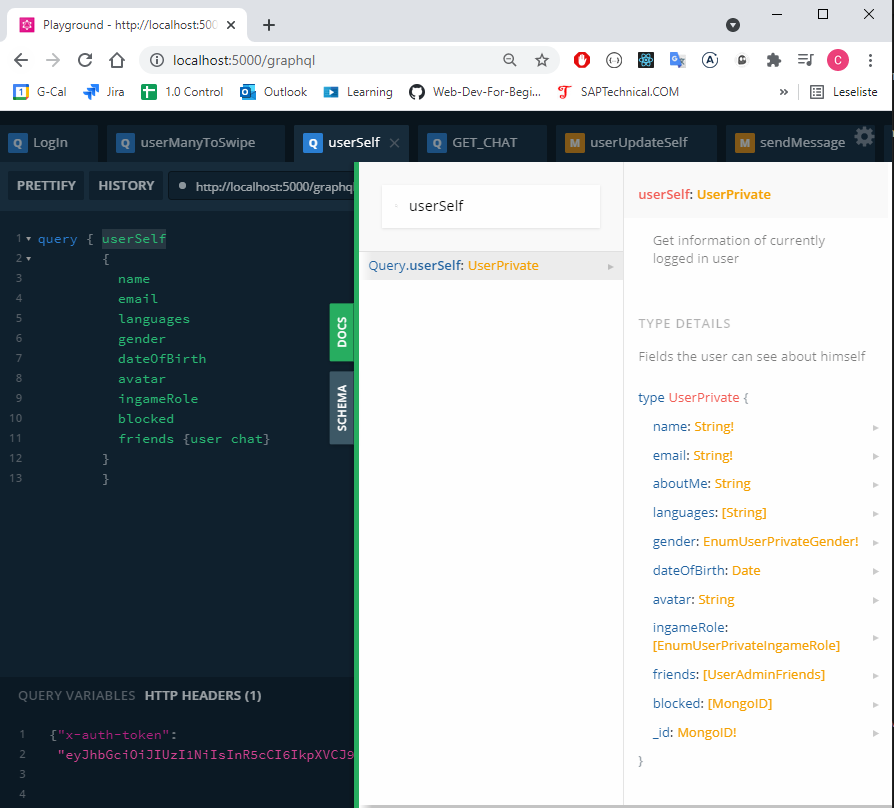
\includegraphics[scale=0.60]{GraphQL_Playground}

\newpage
\textbf{Apollo Client}\\
%Warum haben wir uns dafür entschieden?
Nachdem eine Abfrage exportiert wurde, ist sie bereit, in einer React-Komponente importiert \\ 
und angewendet zu werden.

\begin{lstlisting}
import { GET_MY_INFO } from "./GraphQL/Queries"
import { useQuery } from "@apollo/client"

const { loading, error, data } = useQuery(
GET_MY_INFO,
ContextHeader(token),
)
//Code-Auszug in frontend/src/App.js

\end{lstlisting}
Die Konstante ContextHeader enthält das Token in der Struktur, die erforderlich ist, um die Abfrage nur dann stellen zu können, wenn der Benutzer dazu berechtigt ist.
\\
Sollte das Token undefined, null oder ungültig sein, wird der Server ein Fehler zurückgegeben.
\\ 
Der useQuery Hook liefert ein Ergebnisobjekt, welches eine der folgenden Optionen zurückgibt.
\\
\textbf{loading:}\\
Ein boolescher Wert, der angibt, ob die Abfrage in Bearbeitung ist.
Wenn loading true ist, ist die Anfrage noch nicht abgeschlossen. Typischerweise kann diese Information verwendet werden, um einen Lade-Spinner anzuzeigen.
\\
\textbf{error:}\\
Ein Laufzeitfehler mit den Eigenschaften von GraphQL Errors und network Error.
Dieses enthält Informationen darüber, was bei der Abfrage schief gelaufen ist.
\\
\textbf{date:}\\
Ein Objekt, das das Ergebnis der GraphQL-Abfrage enthält.
\\Es enthält die tatsächlichen Daten vom Server.
\\

AUCH MUTATIONS ZEIGEN\dots
\newpage
\subsection{Axios}
Zusätzlich zu den GraphQL-Abfragen, wurde eine Post-Anfrage mit Axios bereitgestellt.
Mit dieser war es möglich, Bilder auf die S3 Speicher von AWS hochzuladen.

\begin{quote}
Axios ist ein Promise-basierter HTTP-Client für node.js und den browser. Er ist isomorphisch (= kann auf dem server und im browser verwendet weden). Auf der Server-Seite wir das modul http verwendet, während im Browser XMLHttpRequests (ajax) ausgeführt werden.
\end{quote}

\begin{lstlisting}
    function disableBtn() {
        const uploadBtn = document.getElementById("uploadBtn")
        uploadBtn.disabled = true
        uploadBtn.style.background = "#000000"
      }
    
      function fileUploadHandler() {
        errored ? 
         disableBtn()
         /*
        Tritt ein Fehler auf, wird die Abfrage nicht gesendet und der Knopf deaktiviert 
        Ein Fehler tritt auf, wenn die Datei zu gross ist oder oder wenn sie ein ungueltiges  Format hat
        */
        :
        console.log("uploading pic...", file?.name)
        const fd = new FormData()
        /* avatar ist der Name der Datei, die hochgeladen wird
          file ist der zu sendende  Wert */
        fd.append("avatar", file)  
    
        axios
          .post(urlAvatar, fd, {
            headers: {
              "x-auth-token": TOKEN,
            },
          })
          .then((res) => {
            setState((state) => ({ ...state, avatar: res?.data?.location }))    
            //In location finden wir die URL fuer das gerade hochgeladende Bild 
          })
      }\end{lstlisting}

Das HTML-Eingabefeld "input" wurde folgendermaße definiert.
\begin{lstlisting}
    <input type="file" onChange={fileSelectedHandler} />
\end{lstlisting}


Das Format der hochzuladenden Dateien wurde limitiert, damit nur zulässige Dateien an den Server gesendet werden.
\begin{lstlisting}
    const admittedImageFormats = ["png", "jpg", "jpeg"]
\end{lstlisting}

Die Größe der hochzuladenden Datei wurde um 1Mb abgegrenzt.
Durch die Eigenschaft „size“ der ausgewählten Datei konnten wir auf die Größe der Datei zugreifen.
\begin{lstlisting}
    const imageSize = e.target.files[0].size
\end{lstlisting}
 
  %Temporär
  \newpage  
  \section{Glossar}\label{kap_glossar}
  %\newglossaryentry{kiln}
%{
 % name=kiln,
  %description={German: Brennofen (m.);\\Français: fourneau (m.)},
  %plural=kilns
%}

%Make Glossary properly...
%\acrodef{VB}{Visula Basic}

\textbf{Hooks:}\\
...
\textbf{Framework:}\\
...
\textbf{JSX:}\\
Es heißt JSX und ist eine Syntaxerweiterung für JavaScript. Wir empfehlen, sie mit React zu verwenden, um zu beschreiben, wie die Benutzeroberfläche aussehen soll. JSX erinnert vielleicht an eine Template-Sprache, aber es verfügt über die volle Leistungsfähigkeit von JavaScript. JSX erzeugt React-"Elemente"

\textbf{Under-Fetching:}\\

\textbf{Over-Fetching:}\\
Empfang von überschüssigen Daten durch eine Abfrage.
%Reference https://jwt.io/

\textbf{Web Token:}\\
JSON-Web-Tokens sind eine dem Industriestandard RFC 7519 entsprechende Methode zur sicheren Darstellung von Forderungen zwischen zwei Parteien.

\textbf{undefined:}\\
Eine Variable, der kein Wert zugewiesen wurde oder die überhaupt nicht deklariert wurde (nicht deklariert, existiert nicht), ist undefiniert. Eine Methode oder Anweisung gibt auch undefiniert zurück, wenn der ausgewerteten Variablen kein Wert zugewiesen wurde. Eine Funktion gibt undefiniert zurück, wenn kein Wert zurückgegeben wurde.

\textbf{FormData:}\\
Die FormData-Schnittstelle bietet eine einfache Möglichkeit, eine Reihe von Schlüssel/Wert-Paaren zu erstellen, die die Felder eines Formulars und ihre Werte darstellen und mit der XMLHttpRequest.send()-Methode einfach gesendet werden können.

\textbf{Akronyme:}\\

{AWS}{Amazon Web Services}\\
{DOM}{Document Object Model}\\
{API}{Application Programming Interface}\\


 

  \newpage 
  \section{Zusammenfassung und Ausblick}\label{kap_zusammfAusbl}  
   %\input{}
   TEXT FOLGT...
   
     %<MERKKASTEN> (für die eigene Verwendung bitte entfernen
    \vspace{1cm}
 \begin{tcolorbox}[title={Inhalte der \textit{Zusammenfassung und Ausblick}}]
Das Kapitel \textit{Zusammenfassung und Ausblick} enthält folgende formale Aspekte\footnote{Vgl. \cite{BBoJ},S. 6}:
\begin{itemize}
\item Kapitelweise Kurzdarstellung der Inhalte (inklusive Referenzierung auf die Kapitelnummerierung) => Nach dem Motto: \textit{Was wurde wo beschrieben?}
\item Kurzdarstellung \textit{Problem – Lösungsweg – Ergebnisse}
\item Rückkopplung auf die Einleitung: Wurde die Zielstellung der Arbeit und die Fragestellung zufriedenstellend beantwortet?
\item Kritische Bewertung (sofern nicht bereits im Hauptteil geschehen)
\item Offene Probleme
\item Richtung der zukünftigen/möglichen Arbeiten
\item Erläuterung, warum welche Aspekte in der Arbeit nicht erläutert wurden
\end{itemize}
  \end{tcolorbox}
  %</MERKKASTEN>   
   
  % Literaturverzeichnis
   % INFO: Referenzieren auf das Literaturverzeichnis:
   %
   % Befehl: \cite{refmarke}
   % 
   % "refmarke" ist die Angabe in den geschweiften Klammern bei 
   % \bibitem[]{refmarke}. 
   \newpage
    \thispagestyle{empty}
   \section{Quellenverzeichnis}
     \subsection{Literatur}
     \renewcommand{\refname}{} % Literaturverzeichnis ohne Bezeichnung
     % Variante 1: einfaches, manuelles 
     % Literaturverzeichnis
     \begin{thebibliography}{SW11} % 2. {...} => Hier die größte /breiteste Nummer (z.B. 99) oder Kurzbeleg angeben.
       \bibitem[SW11]{SW11} Stickel-Wolf, Christine; Wolf, Joachim (2011): Wissenschaftliches Lernen und Lerntechniken. Erfolgreich studieren–-gewusst wie!. Wiesbaden: Gabler. 
     \end{thebibliography} 
          
     \subsection{Internetquellen}
     \begin{thebibliography}{HR08} % 2. {...} => Hier die größte/breiteste Nummer (z.B. 99) oder Kurzbeleg angeben.
       \bibitem[BBoJ]{BBoJ}Bertelsmeier, Birgit (o. J.): Tipps zum Schrei\-b\-en ei\-n\-er Ab\-sch\-luss\-ar\-beit. Fach\-hoch\-schu\-le Köln-Campus Gummersbach, Institut für Informatik. \url{http://lwibs01.gm.fh-koeln.de/blogs/bertelsmeier/files/2008/05/abschlussarbeitsbetreuung.pdf} (29.10.2013).
        \bibitem[HR08]{HR08} Halfmann, Marion; Rühmann, Hans (2008): Merkblatt zur Anfertigung von Projekt-, Bachelor-, Master- und Diplomarbeiten der Fakultät 10. Fachhochschule Köln-Campus Gummersbach.\url{http://www.f10.fh-koeln.de/imperia/md/content/pdfs/studium/tipps/anleitungda270108.pdf} (29.10.2013).
        \bibitem [V01]{V01} Offizielle Vue-Website: Vergleich zwischen Vue, React und Angular. \url{https://vuejs.org/v2/guide/comparison.html#Preact-and-Other-React-Like-Libraries} (unbekannte Veröffentlichung).
        \bibitem [R01]{R01}Offizielle React-Website: React Hooks. \url{https://reactjs.org/docs/hooks-faq.html#which-versions-of-react-include-hooks}
        \bibitem [A01]{A01}Offizielle Website Apollo für React. \url{https://www.apollographql.com/docs/react/}
        \bibitem [SO01]{SO01}StackOverFlow: Developer Survey 2021. \url{https://insights.stackoverflow.com/survey/2021#section-most-popular-technologies-web-frameworks}
        \bibitem [EE1]{EE1}Elad Elrom: React and Libraries. \url{https://link.springer.com/content/pdf/10.1007%2F978-1-4842-6696-0.pdf}
        \bibitem [SS1]{SS1}Stoyan Stefanov: Durchstarten mit React. \url{https://content-select.com/media/moz_viewer/5d5fc360-478c-4038-ac17-246bb0dd2d03/language:de}
        \bibitem [RH1]{RH1}Red Hat: Was ist GraphQL? \url{https://www.redhat.com/de/topics/api/what-is-graphql}
        \bibitem [PM1]{PM1}Postman: 2020 State of the API Report \url{https://www.postman.com/state-of-api/the-future-of-apis/#the-future-of-apis}
        \bibitem [AX1]{AX1}Offizielle Website Axios \url{https://axios-http.com/}

        
        
     \end{thebibliography} 
  
  % INFO: Biblatex -Ausgabe des  
  % Literaturverzeichnisses (Beispiele):   
  % - \printbibliography => Ausgabe ALLER 
  %   Einträge
  % - \printbibliography[nottype=online]
  %   => Ausgabe der Einträge, bis auf die
  %      "Online"-Einträge
  % - \printbibliography[type=online]     
  %   => Ausgabe nur der "Online"-Einträge  
   %\printbibliography

  % Anhang
  \newpage
  \setcounter{section}{0} % Nummerierung der Gliederungsebene "section" auf 0 setzen
  \renewcommand*\thesection{\Alph{section}} % Nummerierungsart für die Gliederungsebene "section" 
  % auf Großbuchstaben setzen
  \section{Anhang}\label{anhang}
    \subsection{Unterabschnitt von Anhang}\label{subsec_UabsAnhang}
    TEXT FOLGT...
  
  \newpage
  
 % Erklärung über die selbständige Abfassung der Arbeit  
 \pagestyle{empty}
 \section*{Erklärung über die selbständige\\Abfassung der Arbeit} % \section*{...}: das *-Symbol erlaubt, dass dieser
 % Gliederungspunkt nicht ins Inhaltsverzeichnis aufgenommen wird
 \addcontentsline{toc}{section}{Erklärung über die selbständige Abfassung der Arbeit}
 Ich versichere, die von mir vorgelegte Arbeit selbständig verfasst zu haben.
 Alle Stellen, die wörtlich oder sinngemäß aus veröffentlichten oder nicht veröffentlichten Arbeiten anderer entnommen sind,
 habe ich als entnommen kenntlich gemacht.\\ 
 Sämtliche Quellen und Hilfsmittel, die ich für die Arbeit benutzt habe, sind
 angegeben. Die Arbeit hat mit gleichem Inhalt bzw. in wesentlichen Teilen noch keiner anderen Prüfungsbehörde vorgelegen.\\\\
\begin{tabular}{cp{7cm}}
    & \\ 
    & \\ \hline
  \small (Ort, Datum, Unterschrift) & \normalsize \\
  \end{tabular}
  
  %<MERKKASTEN> (für die eigene Verwendung bitte entfernen
    \vspace{1cm}
 \begin{tcolorbox}[title={Hinweise zur obigen \textit{Erklärung}}]
\begin{itemize}
\item Bitte verwenden Sie nur die Erklärung, die Ihnen Ihr \textbf{Prüfungsservice} vorgibt. Ansonsten könnte es passieren, dass Ihre Abschlussarbeit nicht angenommen wird. Fragen Sie im Zweifelsfalle bei Ihrem Prüfungsservice nach.
\item Sie müssen \textbf{alle abzugebende Exemplare} Ihrer Abschlussarbeit unterzeichnen. Sonst wird die Abschlussarbeit nicht akzeptiert. 
\item Ein \textbf{Verstoß} gegen die unterzeichnete \textit{Erklärung} kann u.\,a. die Aberkennung Ihres akademischen Titels zur Folge haben.
\end{itemize}  
  \end{tcolorbox}
  %</MERKKASTEN>   
   
\newpage
% Unbeschriftetes Abschlussblatt (Leere Seite)
\thispagestyle{empty}
\input{leereSeite}


 
\end{document}

